% !TEX root = ../OT4ML.tex

%%%%%%%%%%%%%%%%%%%%%%%%%%%%%%%%%%%%%%%%%%%%%%%%%%%%%%%%%%%%%%%%%%%%%%%%%%%
%%%%%%%%%%%%%%%%%%%%%%%%%%%%%%%%%%%%%%%%%%%%%%%%%%%%%%%%%%%%%%%%%%%%%%%%%%%
%%%%%%%%%%%%%%%%%%%%%%%%%%%%%%%%%%%%%%%%%%%%%%%%%%%%%%%%%%%%%%%%%%%%%%%%%%%
\chapter[Semi-discrete and W1]{Semi-discrete and $\Wass_1$}
\index{semi-discrete!OT}% strictindex
\label{sec-semidiscr-w1}

This chapter develops three computational consequences of duality. Eliminating one potential gives the semi-dual; for discrete measures, this viewpoint leads to auction algorithms, while a continuous source and discrete target lead to Laguerre-cell geometry. The final part specializes duality to $\Wass_1$, where Lipschitz functions and flow fields replace convex potentials. The material connects auction and network-flow methods~\cite{bertsekas1992auction,bertsekas1988dual}, computational geometry~\cite{AurenhammerHA98,Merigot11,merigot2013comparison}, and the Kantorovich--Rubinstein and Beckmann formulations~\cite{kantorovich1958space,Beckmann52}.
\index{Beckmann!formulation}% strictindex
\index{Lipschitz!function}% strictindex
\index{convex!potential}% strictindex
\index{dual!problem}% strictindex

%%%%%%%%%%%%%%%%%%%%%%%%%%%%%%%%%%%%%%%%%%%%%%%%%%%%%%%%%%%%%%%%%%%%%%%%%%%
\section{Semi-dual}\label{sec-semi-dual}
\index{semi-dual}% strictindex

The semi-dual eliminates one potential by an exact $c$-transform. It preserves concavity while removing the explicit pointwise inequality constraint.
\index{c-transform}% strictindex

\paragraph{General measure semi-dual.}
For arbitrary measures, partial maximization converts the constrained two-potential dual into an unconstrained optimization over one function.

The full objective and the result of eliminating its source potential will be used repeatedly in this chapter.
\begin{defn}[Full dual and semi-dual functionals]\label{def-full-dual-functional}
Under the compactness and continuity assumptions of Chapter~\ref{sec-dual}, define
\index{dual!problem}% strictindex
\eql{\label{eq-full-dual-functional}
	\Ee_0(f,g)
	\eqdef
	\begin{cases}
		\displaystyle \int_\Xx f\d\al+\int_\Yy g\d\be,
		& (f,g)\in\Potentials(\c),\\
		-\infty, & \text{otherwise}.
	\end{cases}
}
\eql{\label{eq-semi-dual}
	\Ee(g)
	\eqdef
	\Ee_0(g^{\bar c},g)
	=
	\int_\Xx g^{\bar c}\d\al+\int_\Yy g\d\be.
}
\end{defn}
Thus the dual problem~\eqref{eq-dual-generic} is $\MK_\c(\al,\be)=\max_{f,g}\Ee_0(f,g)$. For fixed $g$, feasibility is equivalent to $f\leq g^{\bar c}$. Since $\al$ is nonnegative, the largest admissible choice $f=g^{\bar c}$ maximizes the objective. Consequently,
\[
	\MK_\c(\al,\be)
	=
	\sup_{g\in\Cc(\Yy)}\Ee(g),
	\qquad
	\Ee(g)=\sup_{f\in\Cc(\Xx)}\Ee_0(f,g).
\]
\index{semi-dual}% strictindex
Partial maximization of a jointly concave objective preserves concavity, so $\Ee$ is concave. The semi-dual is invariant under $g\mapsto g+s$: indeed, $(g+s)^{\bar c}=g^{\bar c}-s$ and both measures have unit mass. Potentials are therefore determined only up to an additive constant, exactly as in the full dual. The main computational advantage is that the semi-dual is unconstrained.

\paragraph{Discrete semi-dual.}
When both measures are discrete, the same elimination produces a finite-dimensional concave objective whose active affine pieces are selected by the discrete $c$-transform.

Let
\[
\al=\sum_{i=1}^n \a_i\de_{x_i},
\qquad
\be=\sum_{j=1}^m \b_j\de_{y_j},
\qquad
\C_{i,j}=c(x_i,y_j),
\]
where $\a\in\RR_+^n$ and $\b\in\RR_+^m$ have the same total mass $M$. We use the same notation for functions and vectors: in the discrete setting,
\[
	\Ee_0(\fD,\gD)
	\eqdef
	\begin{cases}
		\dotp{\fD}{\a}+\dotp{\gD}{\b},
		& \fD\oplus\gD\leq\C,\\
		-\infty, & \text{otherwise}.
	\end{cases}
\]
Eliminating the source potential through the discrete $\bar C$-transform of Remark~\ref{rem-discrete-c-transform} gives
\eql{\label{eq-discrete-semi-dual}
	\MKD_\C(\a,\b)
	=
	\umax{\gD\in\RR^m}\Ee(\gD),
	\qquad
	\Ee(\gD)
	\eqdef
	\Ee_0(\gD^{\bar\C},\gD)
	=
	\sum_{i=1}^n \a_i(\gD^{\bar\C})_i
	+
	\sum_{j=1}^m \b_j\gD_j,
}
with
\[
	(\gD^{\bar\C})_i
	=
	\min_{1\leq j\leq m}(\C_{i,j}-\gD_j).
\]
The function $\Ee$ is concave and piecewise affine. It is invariant under $\gD\mapsto\gD+s\ones_m$, because the two marginals have equal mass. If a tie-breaking rule selects
\[
	\sigma_\gD(i)\in\argmin_j(\C_{i,j}-\gD_j),
\]
then a supergradient is $\b-\widehat\b(\gD)$, where
\[
	\widehat\b_j(\gD)
	\eqdef
	\sum_{i:\,\sigma_\gD(i)=j}\a_i.
\]
Thus the semi-dual supergradient is exactly the mismatch between prescribed target mass and mass currently attracted by each target coordinate. At ties, splitting the corresponding source mass gives the full superdifferential. The auction method developed next specializes this same target-potential formulation to uniform square assignments and couples targeted dual updates with ownership changes.

%%%%%%%%%%%%%%%%%%%%%%%%%%%%%%%%%%%%%%%%%%%%%%%%%%%%%%%%%%%%%%%%%%%%%%%%%%%
\section{Auction Algorithm}
\index{auction algorithm}% strictindex
\label{sec-auction-dual-ascent}

The auction algorithm is derived from coordinate maximization of the semi-dual of the linear assignment problem. Its practical form uses bidder-specific dual-weight updates that cross the selected row's next indifference threshold by $\epsilon$; this controlled relaxation prevents jamming at nonsmooth ties. We follow the particularly transparent account of M\'erigot and Thibert~\cite[Sec.~3.2]{merigot2020optimaltransportalgorithms}, itself based on Bertsekas' auction algorithm and its $\epsilon$-scaling refinement~\cite{bertsekas1981new,bertsekas1988dual,bertsekas1992auction}. Throughout this section, $\C\in\RR^{n\times n}$ and $n\geq2$; the case $n=1$ is immediate. A permutation matrix $\P\in\mathcal P_n^{\mathrm{perm}}$, as defined in Definition~\ref{def-permutation-matrices}, represents the probability coupling $\P/n$.
\index{primal-dual!method}% strictindex
\index{assignment problem}% strictindex

\paragraph{Coordinate ascent and discrete Laguerre cells.}
Auction dual weights give the discrete semi-dual a geometric partition whose cell cardinalities are its coordinate derivatives.

Write $\gD_j$ for the target Kantorovich potential. Specializing~\eqref{eq-discrete-semi-dual} to uniform weights gives
\eql{\label{eq-auction-semidual}
	\Ee(\gD)
	=
	\frac1n\sum_{i=1}^n (\gD^{\bar\C})_i
	+
	\frac1n\sum_{j=1}^n \gD_j,
	\qquad
	(\gD^{\bar\C})_i
	=
	\min_{1\leq j\leq n}(\C_{i,j}-\gD_j).
}
Thus $(\gD^{\bar\C},\gD)$ is dual feasible. This is precisely the discrete $\bar C$-transform of Remark~\ref{rem-discrete-c-transform}, with the same sign convention as in the general and semi-discrete formulations.

The discrete Laguerre cell of target $j$ is
\eql{\label{eq-auction-discrete-laguerre}
	\Laguerre_j^{\rm D}(\gD)
	\eqdef
	\enscond{i\in\range{n}}{
		\C_{i,j}-\gD_j
		\leq
		\C_{i,k}-\gD_k
		\text{ for every }k
	}.
}
These cells can overlap at ties. They are the finite counterpart of the Laguerre cells introduced for the general semi-discrete problem in Definition~\ref{def-laguerre-power-cells}: specifically,~\eqref{eq-auction-discrete-laguerre} is that definition restricted to the source indices. When every row has a unique minimizer, differentiation of~\eqref{eq-auction-semidual} gives
\eql{\label{eq-auction-coordinate-derivative}
	\frac{\partial}{\partial \gD_j}\Ee(\gD)
	=
	\frac{1-\abs{\Laguerre_j^{\rm D}(\gD)}}{n}.
}
Hence an overfull cell calls for a decrease of its dual weight. More generally, Proposition~\ref{prop-assignment-dual-certificate} shows that a perfect matching in the contact graph $i\in\Laguerre_j^{\rm D}(\gD)$ certifies optimality of $\gD$ in~\eqref{eq-auction-semidual}; conversely, assignment duality and complementary slackness produce such a matching at every maximizer. Auction searches for this certificate while moving one coordinate of $\gD$ at a time.

For $i\in\Laguerre_j^{\rm D}(\gD)$, define the bid needed to make row $i$ indifferent between $j$ and its best alternative,
\eql{\label{eq-auction-bid}
	\operatorname{bid}_j(\gD,i)
	\eqdef
	\min_{k\neq j}(\C_{i,k}-\gD_k)
	-
	(\C_{i,j}-\gD_j).
}
When $\Laguerre_j^{\rm D}(\gD)$ is nonempty, the largest maximizing decrement along the negative $j$th coordinate is given by
\(
	\max_{i\in\Laguerre_j^{\rm D}(\gD)}\operatorname{bid}_j(\gD,i)
\)
	\cite[Lem.~20]{merigot2020optimaltransportalgorithms}. This formula explains both the coordinate-ascent interpretation and its weakness: at a tie, even this largest maximizing decrement can vanish, and naive coordinate ascent can jam before reaching a dual maximizer.

\paragraph{Bids and relaxed contacts.}
Exact coordinate maximization can stall at a nonsmooth tie, so auction deliberately moves a bidder $\epsilon$ beyond its next indifference point.

Suppose row $i$ is currently unassigned. Let $j_0$ and $j_1$ be its best and second-best targets for the current dual weights,
\eql{\label{eq-auction-reduced-costs}
	j_0\in\argmin_j(\C_{i,j}-\gD_j),
	\qquad
	j_1\in\argmin_{j\neq j_0}(\C_{i,j}-\gD_j),
}
with fixed deterministic tie-breaking. The bid decreases only the winning dual weight by
\eql{\label{eq-auction-dual-update}
	\Delta_i
	\eqdef
	\operatorname{bid}_{j_0}(\gD,i)+\epsilon
	=
	(\C_{i,j_1}-\gD_{j_1})
	-
	(\C_{i,j_0}-\gD_{j_0})
	+
	\epsilon,
	\qquad
	\gD_{j_0}\leftarrow\gD_{j_0}-\Delta_i.
}
Unlike exact coordinate maximization, this update uses the bid of the selected row rather than the maximum bid over the whole cell. Since $\Delta_i\geq\epsilon$, every selected weight decreases by at least $\epsilon$. After the update, the reduced cost of $j_0$ for row $i$ is exactly $\epsilon$ above that of the unchanged alternative $j_1$. The row nevertheless takes $j_0$; if that target already has an owner, the former owner becomes unassigned. Because of this overshoot, a bid need not increase the nonsmooth semi-dual. Coordinate ascent motivates the update, but $\epsilon$-complementary slackness, rather than monotonicity of the objective, is the invariant that drives the convergence proof.

\begin{defn}[$\epsilon$-complementary slackness]\label{def-auction-eps-cs}
	A partial permutation matrix $\P\in\{0,1\}^{n\times n}$ has at most one nonzero entry in each row and column. Such a matrix and target potential $\gD$ satisfy $\epsilon$-complementary slackness if
	\eql{\label{eq-auction-epsilon-cs}
		\P_{i,j}=1
		\quad\Longrightarrow\quad
		\C_{i,j}-\gD_j
		\leq
		(\gD^{\bar\C})_i+\epsilon.
	}
\end{defn}
The bid~\eqref{eq-auction-dual-update} gives the newly assigned row this property. Decreasing $\gD_{j_0}$ can only make $j_0$ less attractive to rows assigned elsewhere, and its previous owner is removed. Therefore every iteration preserves $\epsilon$-complementary slackness.

\begin{alg}[Bertsekas auction]\label{alg:auction-bidding}
\textbf{Input:} Cost matrix $\C\in\RR^{n\times n}$, tolerance $\epsilon>0$, initial target potential $\gD\in\RR^n$ (default $\gD=0$).

\textbf{Output:} Permutation matrix $\P$ and target potential $\gD$; the source potential is $\gD^{\bar\C}$.

\textbf{Initialize:} Set $\P=0$.

\textbf{While} some row $i$ satisfies $\sum_j\P_{i,j}=0$ \textbf{do}:
\begin{algblock}
\textbf{Choose} any such row $i$.

\textbf{Set} $j_0\in\argmin_j(\C_{i,j}-\gD_j)$ and $j_1\in\argmin_{j\neq j_0}(\C_{i,j}-\gD_j)$.

\textbf{Set} $\Delta\leftarrow(\C_{i,j_1}-\gD_{j_1})-(\C_{i,j_0}-\gD_{j_0})+\epsilon$.

\textbf{Set} $\gD_{j_0}\leftarrow\gD_{j_0}-\Delta$.

\textbf{If} $\P_{i_0,j_0}=1$ for some $i_0$ \textbf{then}:
\begin{algblock}
\textbf{Set} $\P_{i_0,j_0}\leftarrow0$.
\end{algblock}

\textbf{Set} $\P_{i,j_0}\leftarrow1$.
\end{algblock}

\textbf{Return} $\P$ and $\gD$.
\end{alg}

Figure~\ref{fig:dual-auction-progression} shows actual iterates of Algorithm~\ref{alg:auction-bidding} on the planar point clouds of Figure~\ref{fig:matching-2d-cost-exponent}. To expose the dual mechanism geometrically, define the auction reduced costs
\[
\mathrm{r}_{i,j}(\gD)
\eqdef
\C_{i,j}-\gD_j-(\gD^{\bar\C})_i
\geq 0.
\]
At any intermediate state, write
\(
	M\eqdef\{(i,j):\P_{i,j}=1\}
\)
for the current ownership matching. Exact zeros of $\mathrm{r}_{i,j}$ are the discrete Laguerre contacts of row $i$, whereas an edge in $M$ only needs to satisfy $\mathrm{r}_{i,j}(\gD)\leq\epsilon$ by $\epsilon$-complementary slackness.

\begin{figure}[H]
\centering
\setlength{\tabcolsep}{1pt}
\begin{tabular}{ccccc}
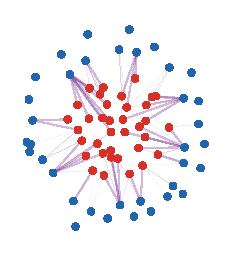
\includegraphics[width=.19\linewidth]{figures/dual-auction-progression/stage-0.pdf} &
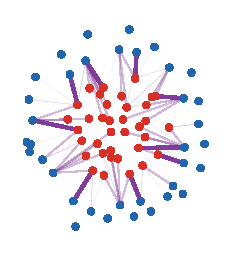
\includegraphics[width=.19\linewidth]{figures/dual-auction-progression/stage-1.pdf} &
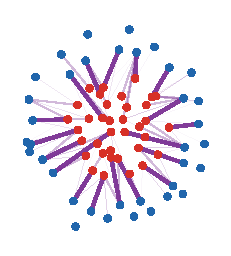
\includegraphics[width=.19\linewidth]{figures/dual-auction-progression/stage-2.pdf} &
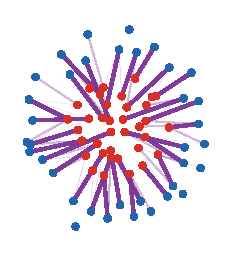
\includegraphics[width=.19\linewidth]{figures/dual-auction-progression/stage-3.pdf} &
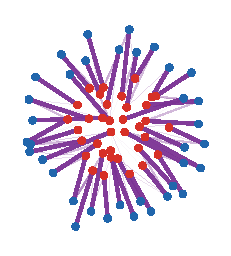
\includegraphics[width=.19\linewidth]{figures/dual-auction-progression/stage-4.pdf} \\[-.1em]
\small $|M|=0$ &
\small $|M|=9$ &
\small $|M|=18$ &
\small $|M|=27$ &
\small $|M|=36$ \\[-.2em]
\footnotesize $0$ bids &
\footnotesize $10$ bids &
\footnotesize $40$ bids &
\footnotesize $98$ bids &
\footnotesize $505$ bids
\end{tabular}
\caption{\emph{Geometric progression of the unit-mass transportation auction.} Thick violet segments form the current partial ownership matching $M$, while the thin translucent segments are the $2n$ unmatched edges with smallest auction reduced costs; exact zero-reduced-cost alternatives are slightly stronger. The panels record the first states with the indicated $|M|$ and report the cumulative number of bids. For $\epsilon=2\times10^{-3}$, the final assignment is reached after $505$ bids and coincides with the exact squared-distance optimum.}
\index{complementary slackness}% strictindex
\label{fig:dual-auction-progression}
\end{figure}

\paragraph{Fixed tolerance.}
For a prescribed tolerance, the relaxed contact condition gives both an optimality certificate and a finite bound on the number of bids.

\begin{prop}[Fixed-$\epsilon$ auction convergence and complexity]\label{prop-auction-termination}
\index{auction algorithm}% strictindex
	Let
	\[
		R_\C\eqdef\max_{i,j}\C_{i,j}-\min_{i,j}\C_{i,j}.
	\]
	Started from $\gD=0$, Algorithm~\ref{alg:auction-bidding} terminates after at most
	\(
		n\bigl(\lfloor R_\C/\epsilon\rfloor+1\bigr)
	\)
	bids. It returns a permutation matrix $\P$ satisfying $\epsilon$-complementary slackness and
	\eql{\label{eq-auction-cost-certificate}
		0
		\leq
		\frac1n\dotp{\C}{\P}
		-
		\umin{\P'\in\mathcal P_n^{\mathrm{perm}}}
		\frac1n\dotp{\C}{\P'}
		\leq
		\epsilon.
	}
	With dense scans for the two smallest reduced costs, the algorithm requires
	\(
		O\bigl(n^2(1+R_\C/\epsilon)\bigr)
	\)
	arithmetic and comparison operations and $O(n^2)$ storage, including $\C$. If $\C$ has integer entries and $\epsilon<1/n$, the returned assignment is exactly optimal.
\end{prop}
\begin{proof}
	At every bid,~\eqref{eq-auction-dual-update} decreases one target potential by at least $\epsilon$. Once a target is assigned, it remains assigned: a later bid can change its owner but never leaves it empty. While the algorithm is incomplete, there is therefore an unassigned target whose potential is still zero. If the selected target $j_0$ is already assigned, comparison with such a zero-potential target gives $\gD_{j_0}\geq-R_\C$; if it is unassigned, its potential is itself zero. Thus a target can be selected at most $\lfloor R_\C/\epsilon\rfloor+1$ times. Summing over the $n$ targets proves finite termination and the bid bound. At termination, every row and column has exactly one nonzero entry, so $\P$ is a permutation matrix.

	The $\epsilon$-complementary-slackness invariant was established above. Summing it over the returned permutation gives the first inequality below. The second is the dual lower bound of Proposition~\ref{prop-assignment-dual-certificate}, applied to the feasible pair $(\gD^{\bar\C},\gD)$:
	\[
		\frac1n\dotp{\C}{\P}
		\leq
		\frac1n\sum_i(\gD^{\bar\C})_i
		+
		\frac1n\sum_j\gD_j
		+
		\epsilon
		\leq
		\umin{\P'\in\mathcal P_n^{\mathrm{perm}}}
		\frac1n\dotp{\C}{\P'}
		+
		\epsilon,
	\]
	which proves~\eqref{eq-auction-cost-certificate}. Each bid scans one row of $\C$ and otherwise uses constant work if the current owner of every target is stored, proving the complexity bound. For integer costs, the unnormalized assignment gap is an integer bounded by $n\epsilon<1$, hence it vanishes.
\end{proof}

\paragraph{$\epsilon$-scaling.}
The cold-start estimate in Proposition~\ref{prop-auction-termination} exposes the limitation of using a single tolerance. A large $\epsilon$ terminates quickly but gives only a coarse certificate, whereas the small $\epsilon$ needed for high accuracy can produce a bid count proportional to $R_\C/\epsilon$. The remedy is continuation: first learn the rough dual-potential landscape with a coarse auction, then decrease the tolerance while retaining that potential.
\index{epsilon-scaling@$\epsilon$-scaling}% strictindex

Algorithm~\ref{alg:auction-epsilon-scaling} starts at the cost scale $\max\{R_\C,\eta\}$ and halves the tolerance until it reaches the requested value $\eta$. Each phase rebuilds the ownership matrix but warm-starts $\gD$ with the preceding phase. Intuitively, the previous complete assignment already certifies approximate contact for this potential; the next phase only needs to refine that contact rather than rediscover the dual landscape from $\gD=0$.

\begin{algH}[Auction with $\epsilon$-scaling]\label{alg:auction-epsilon-scaling}
\textbf{Input:} Cost matrix $\C\in\RR^{n\times n}$, final tolerance $\eta>0$.

\textbf{Output:} Permutation matrix $\P$ and target potential $\gD$; the source potential is $\gD^{\bar\C}$.

\textbf{Initialize:} Set $R_\C\leftarrow\max_{i,j}\C_{i,j}-\min_{i,j}\C_{i,j}$ and $\gD\leftarrow0$.

\textbf{If} $R_\C=0$ \textbf{then}:
\begin{algblock}
\textbf{Return} any permutation matrix $\P$ and $\gD=0$.
\end{algblock}

\textbf{Set} $\epsilon\leftarrow\max\{R_\C,\eta\}$.

\textbf{While} $\epsilon>\eta$ \textbf{do}:
\begin{algblock}
\textbf{Set} $(\P,\gD)\leftarrow\operatorname{Auction}(\C,\epsilon,\gD)$.

\textbf{Set} $\epsilon\leftarrow\max\{\epsilon/2,\eta\}$.
\end{algblock}

\textbf{Set} $(\P,\gD)\leftarrow\operatorname{Auction}(\C,\eta,\gD)$.
\par\noindent
\textbf{Return} $\P$ and $\gD$.
\end{algH}

\begin{prop}[Complexity of $\epsilon$-scaling]\label{prop-auction-epsilon-scaling}
\index{epsilon-scaling@$\epsilon$-scaling}% strictindex
	For a final tolerance $\eta>0$, Algorithm~\ref{alg:auction-epsilon-scaling} returns a permutation matrix satisfying $\eta$-complementary slackness and~\eqref{eq-auction-cost-certificate} with $\epsilon$ replaced by $\eta$. If $R_\C>0$, it uses at most
	\[
		1+\left\lceil\log_2^+\!\left(\frac{R_\C}{\eta}\right)\right\rceil
	\]
	auction phases, where $\log_2^+(s)\eqdef\max\{0,\log_2 s\}$. Its dense worst-case complexity is
	\[
		O\left(n^3\left(1+\log_+\frac{R_\C}{\eta}\right)\right),
		\qquad
		\log_+(s)\eqdef\max\{0,\log s\}.
	\]
	When $R_\C=0$, the algorithm terminates immediately. If $\C$ has integer entries and $\eta<1/n$, the returned assignment is exactly optimal.
\end{prop}
\begin{proof}
	Assume $R_\C>0$. The first tolerance is $\epsilon_0=\max\{R_\C,\eta\}$. If $\epsilon_0=\eta$, Proposition~\ref{prop-auction-termination} directly gives the claim with one phase. Otherwise, the first phase starts from the zero potential and costs $O(n^2)$ operations because $R_\C/\epsilon_0=1$.

	Consider a later phase with tolerance $\epsilon$, initialized from a target potential produced at tolerance $\lambda$. The preceding complete assignment satisfies $\lambda$-complementary slackness for this potential. Expressed in the present dual-potential convention, the warm-start estimate of~\cite[Lem.~25]{merigot2020optimaltransportalgorithms} shows that the new phase decreases each component of $\gD$ by at most $n(\lambda+\epsilon)$. Since every bid decreases one component by at least $\epsilon$, the phase performs at most
	\[
		n^2\left(1+\frac{\lambda}{\epsilon}\right)
	\]
	bids. Consecutive tolerances in Algorithm~\ref{alg:auction-epsilon-scaling} satisfy $\lambda/\epsilon\leq2$, so a warm-started phase uses $O(n^2)$ bids and $O(n^3)$ dense operations.

	Halving from $R_\C$ to $\eta$ gives the announced phase count. The final phase enforces $\eta$-complementary slackness, and Proposition~\ref{prop-auction-termination} gives the $\eta$-optimality certificate. Its integer-cost conclusion also applies with $\epsilon=\eta$.
\end{proof}

Compared with a single $\eta$-auction started from zero, whose dense bound grows as $O(n^2(1+R_\C/\eta))$, scaling replaces the linear accuracy factor by a logarithmic number of $O(n^3)$ phases. This is a high-accuracy guarantee rather than an unconditional speedup: at coarse tolerances the cold-start bound can be smaller, while the scaling bound improves it once $R_\C/\eta$ is large compared with $n\bigl(1+\log_+(R_\C/\eta)\bigr)$. For integer costs, choosing $\eta<1/n$ gives an exact assignment with complexity $O\bigl(n^3(1+\log_+(nR_\C))\bigr)$.

\begin{rem}[$\epsilon$-scaling and relation with Sinkhorn]
	Sinkhorn uses a superficially similar continuation parameter, but its role is different. Entropy replaces the hard minimum in the semi-dual by a smooth log-sum-exp, whereas auction retains the hard discrete transform and relaxes only the contact condition. Sinkhorn evolves a dense coupling by smooth block maximization; auction maintains a partial permutation matrix through dual-weight bids and ownership changes.
\index{Sinkhorn!algorithm}% strictindex
\index{entropic!regularization}% strictindex
\index{log-sum-exp}% strictindex
\end{rem}


%%%%%%%%%%%%%%%%%%%%%%%%%%%%%%%%%%%%%%%%%%%%%%%%%%%%%%%%%%%%%%%%%%%%%%%%%%%
\section{Semi-discrete}
\index{semi-discrete!OT}% strictindex


The semi-discrete case is the setting where dual potentials become weights of Laguerre cells. This gives both geometry and algorithms for quantization and density fitting.
\index{dual!potential}% strictindex
\index{Laguerre cell}% strictindex

\paragraph{Discrete target and Laguerre cells.}
\index{discrete!target}% strictindex

A case of particular interest is when
\(
\be = \sum_{j=1}^m \b_j \de_{y_j}
\)
has distinct atoms and positive weights. Zero-weight atoms can simply be removed. The same construction applies when $\al$ is discrete by exchanging the roles of $\al$ and $\be$.
%
One can adapt Definition~\ref{def-c-transform} of the $\bar c$-transform to this setting by restricting the minimization to the finite support $\{y_j\}_{j=1}^m$ of $\be$. Equivalently, one applies the same definition with the discrete target space $\Y=\{y_j\}_{j=1}^m$ and identifies a vector $\gD\in\RR^m$ with the function $g:\Y\to\RR$ defined by $g(y_j)=\gD_j$:
\index{c-transform}% strictindex
\eql{\label{eq-disc-c-transfo}
	\foralls \gD \in \RR^m, \;
	\foralls x \in \Xx, \quad
	\gD^{\bar \c}(x) \eqdef \umin{j \in \range{m}} \c(x,y_j) - \gD_j.
}
This transform maps a vector $\gD$ to a continuous function $\gD^{\bar \c} \in \Cc(\Xx)$ because it is the minimum of finitely many continuous functions.

Crucially, using the discrete $\bar c$-transform, when $\be$ is a discrete measure, yields a finite-dimensional optimization,
\eql{\label{eq-semi-dual-discr}
\index{semi-dual}% strictindex
		\MK_\c(\al,\be) =
			\umax{\gD \in \RR^m}
				\Ee(\gD) \eqdef \Ee_0(\gD^{\bar\c},\gD) =
				\int_\Xx \gD^{\bar \c}(x) \d\al(x) + \sum_j \gD_j \b_j.
}
The objective satisfies $\Ee(\gD+s\ones)=\Ee(\gD)$ for every $s\in\RR$. One may therefore impose the gauge $\sum_j\gD_j=0$ without changing the problem. The geometric object encoded by the dual weights is a weighted nearest-neighbor diagram: each source point is assigned to a target atom realizing the discrete $\bar c$-transform.

\begin{defn}[Laguerre cells and power diagrams]\label{def-laguerre-power-cells}
\index{Laguerre cell}% strictindex
\index{power diagram}% strictindex
\index{dual!weight}% strictindex
	For sites $(y_j)_{j=1}^m$ and weights $\gD\in\RR^m$, the Laguerre cell associated with $y_j$ is
	\eql{\label{eq-laguerre-cells}
		\Laguerre_{j}(\gD) \eqdef \enscond{x \in \Xx}{ \foralls j' \neq j, \c(x,y_j) - \gD_j \leq \c(x,y_{j'}) - \gD_{j'} }.
	}
	The cells cover $\Xx$; after arbitrary tie-breaking on common boundaries, they induce a disjoint partition. When $c(x,y)=\norm{x-y}^2$, this Laguerre decomposition is also called a power diagram. If $\gD$ is constant, it reduces to the ordinary Voronoi diagram.
\end{defn}
For quadratic costs, varying the dual weights moves the walls between adjacent cells while keeping them parallel; this is the geometric mechanism by which the cell masses are adjusted.
\index{cell mass}% strictindex
\index{quadratic!cost}% strictindex
\index{dual!weight}% strictindex
%
Figure~\ref{fig:semidiscrete-laguerre-cells} follows this adjustment from unweighted Voronoi cells to a power diagram whose cell masses match the prescribed discrete target weights.

\begin{figure}[H]
\centering
\begin{tabular}{@{}ccc@{}}
\small zero weights &
\small intermediate weights &
\small balanced cells \\[-.15em]
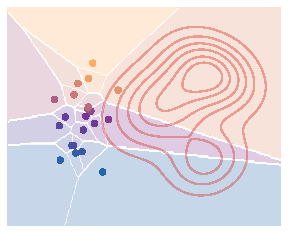
\includegraphics[width=.30\linewidth]{figures/semidiscrete-laguerre-cells/voronoi.pdf} &
\index{Laguerre cell}% strictindex

\includegraphics[width=.30\linewidth]{figures/semidiscrete-laguerre-cells/weighted.pdf} &

\includegraphics[width=.30\linewidth]{figures/semidiscrete-laguerre-cells/balanced.pdf}
\end{tabular}
\caption{\emph{Laguerre cells for semi-discrete quadratic transport.} The red contours show a continuous source density $\al$ given by a three-component Gaussian mixture on the right. The twenty-one colored circular sites are the atoms of the discrete target $\be$ sampled from a compact Gaussian cloud on the left; each site color matches its Laguerre cell. Starting from ordinary Voronoi cells, semi-dual weight updates deform the cells so that the $\al$-mass captured by each cell approaches the prescribed target mass.}
\index{Gaussian!mixture}% strictindex
\index{semi-discrete!OT}% strictindex
\index{Voronoi cell}% strictindex
\index{dual!weight}% strictindex
\index{semi-dual}% strictindex
\label{fig:semidiscrete-laguerre-cells}
\end{figure}

\paragraph{Mass balance.}
\index{mass!balance}% strictindex

This gives the convenient semi-dual form
\eql{\label{eq-semi-disc-energy}
	\Ee(\gD) = \sum_{j=1}^m \int_{\Laguerre_{j}(\gD)} \pa{ c(x,y_j) - \gD_j } \d\al(x) + \dotp{\gD}{\b}.
}
The following proposition provides a formula for the gradient of this concave function.

\begin{prop}[Gradient of the semi-discrete dual]\label{prop-semidiscrete-dual-gradient}
\index{semi-discrete!dual}% strictindex
If the minimizing index in~\eqref{eq-disc-c-transfo} is unique for $\al$-almost every $x$, then $\Ee$ is differentiable at $\gD$ and
\index{zero mass}% strictindex
\index{Laguerre cell}% strictindex
\eq{
	\foralls j \in \range{m}, \quad
	\nabla\Ee(\gD)_j = \b_j - \int_{\Laguerre_{j}(\gD)} \d\al.
}
\end{prop}
\begin{proof}
	For $\al$-almost every $x$, the minimizing index in $\min_j c(x,y_j)-\gD_j$ is unique. If this index is $j(x)$, then the directional derivative in a direction $h\in\RR^m$ is
	\[
		\left.\frac{\d}{\d t}\right|_{t=0}
		\min_j \bigl(c(x,y_j)-(\gD_j+t h_j)\bigr)
		=
		-h_{j(x)}.
	\]
	The corresponding difference quotients are bounded by $\norm{h}_\infty$. Dominated convergence therefore gives
	\[
		\d\Ee(\gD)[h]
		=
		-\sum_j h_j\int_{\Laguerre_j(\gD)}\d\al
		+\sum_j h_j\b_j,
	\]
	which is the announced gradient formula.
\end{proof}

Because the gradient components sum to zero, gradient ascent preserves the chosen gauge. At a differentiable maximizer, first-order optimality gives
\(
\al(\Laguerre_j(\gD))=\b_j
\)
for every $j$. Conversely, if these identities hold, the piecewise-constant map $T(x)=y_j$ on $\Laguerre_j(\gD)$ pushes $\al$ onto $\be$. Its graph lies in the contact set
\(
\gD^{\bar c}(x)+\gD_j=c(x,y_j),
\)
so complementary slackness, Proposition~\ref{prop-continuous-complementary-slackness}, proves that $T$ and $\gD$ are optimal. For the quadratic cost, uniqueness of the map follows from Brenier's theorem when $\al$ has a density.
\index{optimality!first-order}% strictindex
\index{Brenier!theorem}% strictindex
\index{quadratic!cost}% strictindex
\index{semi-discrete!OT}% strictindex


Figure~\ref{fig:semidiscrete-weight-gradient-cells} makes the sign of this gradient geometric. Increasing a weight lowers the corresponding power distance and expands the associated Laguerre cell; decreasing it shrinks the cell. The dotted outline marks the balanced cell, so the semi-dual ascent can be read as a mass-balancing procedure on a power diagram.
\index{dual!weight}% strictindex
\index{Laguerre cell}% strictindex
\index{cell mass}% strictindex

\begin{figure}[H]
\centering
\begin{tabular}{@{}ccc@{}}
\small underweight &
\small balanced &
\small overweight \\[-.15em]
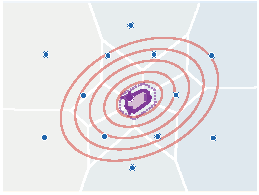
\includegraphics[width=.30\linewidth]{figures/semidiscrete-weight-gradient-cells/underweight.pdf} &

\includegraphics[width=.30\linewidth]{figures/semidiscrete-weight-gradient-cells/balanced.pdf} &
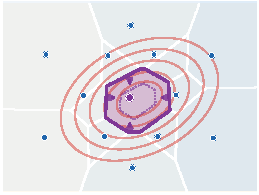
\includegraphics[width=.30\linewidth]{figures/semidiscrete-weight-gradient-cells/overweight.pdf}
\end{tabular}
\caption{\emph{Dual weights control Laguerre cell masses in the semi-discrete quadratic problem.} The same blue target sites and red Gaussian source density are used in all panels; only the highlighted violet weight is changed. The dotted violet outline is the balanced cell. If the highlighted cell has too little source mass, then $\b_j-\al(\Laguerre_j(\gD))>0$ and the ascent update increases the weight, expanding the cell outward. If it has too much mass, the update decreases the weight, shrinking it inward. At balance, the cell mass matches the prescribed target mass and the first-order update vanishes.}
\index{semi-discrete!dual}% strictindex
\index{power diagram}% strictindex
\index{dual!gradient}% strictindex
\label{fig:semidiscrete-weight-gradient-cells}
\end{figure}

\begin{alg}[Semi-discrete Laguerre ascent]\label{alg:semidiscrete-laguerre-ascent}
\textbf{Input:} Source measure $\al$, target atoms $(y_j,\b_j)$, cost $c$, steps $(\tau_k)_{k=0}^{K-1}$, tolerance $\mathrm{tol}$, iteration budget $K\geq1$.

\textbf{Output:} Semi-discrete dual weights $\gD$ and Laguerre cells.
\index{Laguerre cell}% strictindex

\textbf{Initialize:} Set $\gD^{(0)}=0$.

\textbf{For} $k=0,\ldots,K-1$ \textbf{do}:
\begin{algblock}

\textbf{Compute cells:}
\(\Laguerre_j(\gD^{(k)}) = \enscond{x}{c(x,y_j)-\gD^{(k)}_j\leq c(x,y_\ell)-\gD^{(k)}_\ell\quad\forall \ell}.\)

\textbf{Compute masses:}
\(m_j^{(k)}=\int_{\Laguerre_j(\gD^{(k)})}\d\al .\)

\textbf{If} $\max_j\abs{m_j^{(k)}-\b_j}\leq\mathrm{tol}$ \textbf{then}:
\begin{algblock}
\textbf{Return} $\gD^{(k)}$ and $\bigl(\Laguerre_j(\gD^{(k)})\bigr)_{j=1}^m$.
\end{algblock}

\textbf{Update}
\(\gD^{(k+1)} = \gD^{(k)}+\tau_k\bigl(\b-m^{(k)}\bigr).\)
\end{algblock}
\algreturnskip
\textbf{Compute} $\bigl(\Laguerre_j(\gD^{(K)})\bigr)_{j=1}^m$.

\textbf{Return} $\gD^{(K)}$ and these cells.
\end{alg}

The quadratic power diagrams of Definition~\ref{def-laguerre-power-cells} have polyhedral cells and can be computed efficiently using computational-geometry algorithms~\cite{aurenhammer1987power,AurenhammerHA98,Merigot11}. Expanding the squared distance shows that the active cell at $x$ minimizes the affine function
\(
x\mapsto -2\dotp{x}{y_j}+\norm{y_j}^2-\gD_j.
\)
The lower envelope of these affine functions produces the power diagram, while the lower convex hull of the lifted sites $(y_j,\norm{y_j}^2-\gD_j)$ produces its dual regular triangulation. For a planar source domain, the lift lives in $\RR^3$; Chan's output-sensitive three-dimensional convex-hull algorithm computes a hull with $Q$ vertices in $O(m\log Q)$ time~\cite{chan1996optimal}. A three-dimensional source requires a four-dimensional hull and therefore does not fall under that particular complexity bound.
\index{power diagram}% strictindex

\paragraph{Stochastic optimization.}
\index{stochastic!optimization}% strictindex

The semi-discrete formulation~\eqref{eq-semi-disc-energy} is useful because the objective is an expectation with respect to $\al$,
\index{semi-discrete!OT}% strictindex
\eql{\label{eq-semi-disc-energy-entropy}
	\Ee(\gD)
	=
	\int_\Xx E(\gD,x)\d\al(x)
	=
	\EE_X(E(\gD,X)),
	\qquad
	E(\gD,x)\eqdef \gD^{\bar c}(x)+\dotp{\gD}{\b}.
}
Here $X\sim\al$. Away from cell boundaries, the stochastic gradient of the integrand is
\index{stochastic!gradient}% strictindex
\[
	\nabla_{\gD}E(\gD,x)
	=
	\left(\b_j-\ones_{\Laguerre_j(\gD)}(x)\right)_{j=1}^m,
\]
which is an unbiased estimator of $\nabla\Ee(\gD)$ when cell boundaries have $\al$-measure zero. One can therefore maximize~\eqref{eq-semi-disc-energy} without first discretizing $\al$: the measure is used as a black box from which independent samples are drawn, a natural setup in high-dimensional statistics and machine learning.

Starting from $\gD^{(0)}=0$, stochastic gradient ascent draws $x_\ell\sim\al$ and performs
\index{stochastic!gradient}% strictindex
\eql{\label{eq-sgd}
	\gD^{(\ell+1)}
	\eqdef
	\gD^{(\ell)}+\tau_\ell\nabla_{\gD}E(\gD^{(\ell)},x_\ell).
}
Equivalently, if
\[
	j_\ell\in\argmin_j\bigl(c(x_\ell,y_j)-\gD_j^{(\ell)}\bigr),
\]
then the coordinate update is
\[
	\gD_j^{(\ell+1)}
	=
	\gD_j^{(\ell)}
	+
	\tau_\ell\bigl(\b_j-\ones_{\{j=j_\ell\}}\bigr).
\]
The stochastic supergradient has zero coordinate sum, so the iterates preserve the gauge $\sum_j\gD_j=0$. For almost-sure stochastic-approximation convergence, one typically chooses
\eql{\label{eq-step-size-sgd}
	\sum_{\ell=0}^{+\infty}\tau_\ell=+\infty,
	\qquad
	\sum_{\ell=0}^{+\infty}\tau_\ell^2<+\infty,
}
for instance $\tau_\ell=\tau_0(1+\ell/\ell_0)^{-q}$ with $1/2<q\leq1$. A finite-horizon $O(L^{-1/2})$ guarantee instead uses averaging and a horizon-dependent step, as made precise next.
\index{rate!sublinear}% strictindex

\begin{prop}[Averaged stochastic semi-dual rate]\label{prop-semidiscrete-sgd-rate}
	Let $\gD^\star$ maximize $\Ee$, set $R=\norm{\gD^{(0)}-\gD^\star}_2$, and suppose the stochastic supergradients are conditionally unbiased and satisfy $\norm{\nabla_\gD E(\gD,x)}_2\leq G$. For a horizon $L\geq1$, use the constant step $\tau=R/(G\sqrt L)$ and the average $\bar\gD_L=L^{-1}\sum_{\ell=0}^{L-1}\gD^{(\ell)}$. If $R=0$, the conclusion is immediate; otherwise,
	\[
		\Ee(\gD^\star)-\EE\bigl[\Ee(\bar\gD_L)\bigr]
		\leq
		\frac{RG}{\sqrt L}.
	\]
\end{prop}
\begin{proof}
	Conditionally on $\gD^{(\ell)}$, the stochastic supergradient is unbiased. Concavity and the squared-distance recursion give
	\[
		2\tau\,\EE\!\left[\Ee(\gD^\star)-\Ee(\gD^{(\ell)})\right]
		\leq
		\EE\norm{\gD^{(\ell)}-\gD^\star}_2^2
		-
		\EE\norm{\gD^{(\ell+1)}-\gD^\star}_2^2
		+
		\tau^2G^2.
	\]
	Summing from $0$ to $L-1$, discarding the final nonnegative squared distance, and using concavity at $\bar\gD_L$ yields
	\[
		\Ee(\gD^\star)-\EE\!\left[\Ee(\bar\gD_L)\right]
		\leq
		\frac{R^2}{2\tau L}+\frac{\tau G^2}{2}.
	\]
	The stated choice of $\tau$ gives the result.
\end{proof}

Here one may take $G\leq2$ because each sample supergradient is $\b-e_{j_\ell}$. This stochastic viewpoint is one of the main algorithmic advantages of the semi-discrete formulation~\cite{Merigot11,genevay2016stochastic}.
\index{semi-discrete!OT}% strictindex

\begin{alg}[Stochastic semi-discrete ascent]\label{alg:semidiscrete-stochastic-ascent}
\textbf{Input:} Source sampler $x\sim\al$, target atoms $(y_j,\b_j)$, steps $(\tau_\ell)_{\ell=0}^{L-1}$, iteration count $L$.

\textbf{Output:} Stochastic semi-discrete dual weights $\gD$.

\textbf{Initialize:} Set $\gD^{(0)}=0$.

\textbf{For} $\ell=0,\ldots,L-1$ \textbf{do}:
\begin{algblock}

\textbf{Draw} $x_\ell\sim\al$.

\textbf{Set} \(j_\ell=\min\argmin_j\bigl(c(x_\ell,y_j)-\gD_j^{(\ell)}\bigr)\).

\textbf{For} $j=1,\ldots,m$ \textbf{do}:
\begin{algblock}
\(\gD_j^{(\ell+1)} = \gD_j^{(\ell)} + \tau_\ell\bigl(\b_j-\ones_{\{j=j_\ell\}}\bigr).\)
\end{algblock}
\end{algblock}
\algreturnskip
\textbf{Return} $\bar\gD_L=L^{-1}\sum_{\ell=0}^{L-1}\gD^{(\ell)}$.
\end{alg}


%%%%%%%%%%%%%%%%%%%%%%%%%%%%%%%%%%%%%%%%%%%%%%%%%%%%%%%%%%%%%%%%%%%%%%%%%%%
\section{Optimal Quantization}
\index{quantization!optimal}% strictindex
\label{sec-optimal-quantization}

Optimal quantization asks for the best discrete approximation of a measure by $m$ codepoints. It is the geometric core of vector quantization, compression and $k$-means clustering.

\paragraph{Free masses and prescribed weights.}
\index{quantization!non-uniform weights}% strictindex
The classical free-mass problem optimizes both the codepoint positions and their probabilities. Prescribing the weights gives a different approximation problem, whose equal-weight specialization is treated below.

The free-mass approximation is the basic quantization problem.
\begin{defn}[Optimal quantization problem]\label{def-optimal-quantization}
For $\al\in\Pp_p(\RR^d)$ and $m\in\NN\setminus\{0\}$, define
\eql{\label{eq-optimal-quantization}
	\Qq_m(\al)
	\eqdef
	\umin{Y=(y_j)_{j=1}^m,\ \b\in\simplex_m}
	\Wass_p\left(\al,\sum_{j=1}^m \b_j\de_{y_j}\right).
}
Zero weights and coincident codepoints are allowed, so the approximating measure has at most $m$ atoms.
\end{defn}
This problem is classical in approximation theory and information theory~\cite{graf2000foundationsquantization,Lloyd82}.

In~\eqref{eq-optimal-quantization}, one optimizes both the codepoint positions $Y=(y_j)_j$ and the weights $\b\in\simplex_m$. The equal-weight case, $\b_j=1/m$, is especially important for particle approximations and is isolated at the end of this section.

\begin{prop}[Quantization rate and curse of dimensionality]\label{prop-quantization-rate}
\index{quantization!rate}% strictindex
\index{curse of dimensionality}% strictindex
	Let $\al$ be supported in a bounded subset $\Omega\subset\RR^d$ and assume that $\al=\rho\,\d x$ with $\rho\leq\rho_+<+\infty$. Then, for fixed $p\geq1$, there exist constants $0<c\leq C<+\infty$ such that
	\[
		c\,m^{-1/d}
		\leq
		\Qq_m(\al)
		\leq
		C\,m^{-1/d}.
	\]
\end{prop}
\begin{proof}
	Enclose $\Omega$ in a cube. With $k=\lfloor m^{1/d}\rfloor$, subdivide this cube into $k^d\leq m$ congruent subcubes and place one codepoint in each subcube meeting $\Omega$. Every source point then lies within distance $C/k\leq C'm^{-1/d}$ of a codepoint. The nearest-codepoint coupling proves the upper bound; unused codepoints may be assigned zero mass.

	For the lower bound, fix any set $Y$ of at most $m$ codepoints and write $d_Y(x)=\min_j\norm{x-y_j}$. If $\omega_d$ is the volume of the Euclidean unit ball, then
	\(
	\al(\{d_Y\leq t\})\leq \rho_+m\omega_dt^d.
	\)
	Set $t_0=(2\rho_+m\omega_d)^{-1/d}$. Then $\al(\{d_Y>t\})\geq1/2$ for $0<t<t_0$, and the layer-cake formula gives
	\[
		\int d_Y(x)^p\d\al(x)
		=
		\int_0^{+\infty} p t^{p-1}\al(\{d_Y>t\})\d t
		\geq
		\frac{t_0^p}{2}
		\simeq
		c m^{-p/d}.
	\]
	Taking the $p$-th root and minimizing over $Y$ proves the lower bound.
\end{proof}

This deterministic rate mirrors the empirical OT sample-complexity rate: both are governed by the spacing $m^{-1/d}$ of points in dimension $d$. Quantization is best-case and deterministic, while empirical OT is random, but both display the same curse of dimensionality. Zador's theorem refines this comparison by identifying the sharp asymptotic constant and the limiting density of optimal codepoints~\cite{graf2000foundationsquantization}.
\index{empirical!OT}% strictindex
\index{curse of dimensionality}% strictindex
\index{sample complexity}% strictindex
For fixed codepoints $Y$, the powered transport cost
\(
\b\mapsto\Wass_p^p(\al,\sum_j\b_j\de_{y_j})
\)
is convex because it is an optimal value of a linear program with affine marginal constraints. This statement need not hold for its $p$-th root $\Wass_p$. The dependence on $Y$ is non-convex and is generally computationally hard. The rest of this section distinguishes the free-mass Lloyd reduction from the fixed-weight geometry underlying finite-particle $\Wass_2$ gradient flows.
\index{quadratic!cost}% strictindex

\paragraph{Lloyd algorithm.}
\index{Lloyd!algorithm}% strictindex
The computational appeal of quantization comes from splitting the non-convex search over sites into two elementary operations. For fixed sites, the optimal assignment is purely local: each point is sent to one of its nearest sites, and the resulting cells are Voronoi cells. This is the assignment step behind Lloyd's algorithm and the $k$-means method.

\begin{prop}[Free masses give Voronoi cells]\label{prop-free-masses-voronoi}
\index{mass!free}% strictindex
\index{Voronoi cell}% strictindex
	For the cost $c(x,y)=d(x,y)^p$, fix distinct codepoints $Y=(y_j)_{j=1}^m$. Duplicate codepoints can be merged beforehand. Minimizing over the weights $\b\in\simplex_m$ gives
	\[
		\min_{\b\in\simplex_m}
		\Wass_p^p\left(\al,\sum_j \b_j\de_{y_j}\right)
		=
		\int_\X \min_{1\leq j\leq m} c(x,y_j)\d\al(x).
	\]
	An optimal coupling is induced by sending each $x$ to a nearest codepoint. The corresponding cells are the Voronoi cells
\index{optimal coupling}% strictindex
\index{Voronoi cell}% strictindex
	\[
		\VV_j(Y)
		\eqdef
		\enscond{x}{\foralls j',\ c(x,y_j)\leq c(x,y_{j'})},
	\]
	up to arbitrary tie-breaking on common boundaries.
\end{prop}
\begin{proof}
	For any coupling between $\al$ and a measure supported on $Y$, the conditional destination of a point $x$ belongs to $Y$, hence its conditional cost is at least $\min_j c(x,y_j)$. Integrating gives the lower bound. Conversely, choose a measurable nearest-codepoint map $T_Y(x)\in\argmin_j c(x,y_j)$, breaking ties measurably, and set $\b_j=\al(T_Y^{-1}(y_j))$. Then $(T_Y)_\sharp\al=\sum_j \b_j\de_{y_j}$ and the induced transport reaches the displayed lower bound.
\end{proof}

Consequently, the quantization energy can be written in the nearest-centroid form
\index{quantization!energy}% strictindex
\[
	\Qq_m(\al)^p
	=
	\min_Y \Ff(Y),
	\qquad
	\Ff(Y)
	\eqdef
	\int_\X \min_{1\leq j\leq m} c(x,y_j)\d\al(x).
\]
At a differentiability point of this energy, any local minimizer with nonempty cells satisfies the centroid condition
\[
	y_j
	\in
	\uargmin{y}
	\int_{\VV_j(Y)} c(x,y)\d\al(x).
\]
For the squared Euclidean cost, this becomes the fixed-point equation
\[
	y_j
	=
	\frac{\int_{\VV_j(Y)} x\d\al(x)}
	{\int_{\VV_j(Y)} \d\al}.
\]
Lloyd's algorithm, also known as the $k$-means algorithm, iterates this fixed point: assign points to nearest sites, then replace each site by the centroid of its cell~\cite{Lloyd82}. The assignment step minimizes the cost for fixed sites, and the centroid step minimizes it for the resulting fixed partition; hence the objective cannot increase. Since the problem is non-convex in $Y$, this descent does not guarantee a global minimizer and may stop at a stationary configuration or local minimum. Good seeding matters. For a finite data set with squared Euclidean loss, $k$-means++ gives an expected logarithmic approximation guarantee~\cite{ArthurVassilvitskii2007}.

\paragraph{Continuous Lloyd flow.}
\index{Lloyd!flow}% strictindex
\index{centroidal Voronoi tessellation}% strictindex
There is also an infinitesimal version of Lloyd's fixed point, but it should first be understood on finite labelled configurations. Assume that \(c(x,y)=\norm{x-y}^2\) and that \(\al\) does not charge Voronoi boundaries. For a configuration \(Y\), define, on nonempty cells,
\[
	a_j(Y)=\al(\VV_j(Y)),
	\qquad
	b_j(Y)=\frac{1}{a_j(Y)}\int_{\VV_j(Y)}x\,\d\al(x)
\]
as the cell mass and centroid. Empty cells are singular points of the vector field; one either freezes them, as in the algorithm below, or reseeds them. The relaxed Lloyd step
\[
	y_j^{(k+1)}=y_j^{(k)}+\tau\big(b_j(Y^{(k)})-y_j^{(k)}\big),
	\qquad 0<\tau\leq 1,
\]
is the explicit-Euler discretization of the cell-mass preconditioned gradient flow of the quantization energy \(\Ff\),
\[
	\dot y_j(t)=b_j(Y_t)-y_j(t).
\]
Indeed, at differentiability points of \(\Ff\), the envelope theorem gives
\[
	\nabla_{y_j}\Ff(Y)
	=
	2\int_{\VV_j(Y)}(y_j-x)\d\al(x)
	=
	2a_j(Y)(y_j-b_j(Y)),
\]
so that
\[
	\dot y_j(t)
	=
	-\frac{1}{2a_j(Y_t)}\nabla_{y_j}\Ff(Y_t).
\]
Equivalently, this is the gradient flow of \(\Ff\) for the site metric \(g_Y(U,V)=2\sum_j a_j(Y)\dotp{u_j}{v_j}\); it is not the unweighted Euclidean gradient flow unless the masses are absorbed into the time step. Along smooth portions of the flow,
\[
	\frac{\d}{\d t}\Ff(Y_t)
	=
	-2\sum_j a_j(Y_t)\norm{b_j(Y_t)-y_j(t)}^2
	\leq 0.
\]
If \(\eta_t=\sum_j w_j\de_{y_j(t)}\) carries fixed positive weights, independent of the Voronoi masses \(a_j(Y_t)\), Proposition~\ref{prop-lagrangian-flow-continuity} turns this labelled particle ODE into the weak continuity equation
\[
	\partial_t\eta_t+\diverg(v_t\eta_t)=0,
	\qquad
	v_t(y_j(t))=b_j(Y_t)-y_j(t),
\]
in the sense of the measure evolutions of Section~\ref{sec-dynamic-optimal-transport}. The weights \(w_j\) in this transport equation are auxiliary weights for the moving labelled particles; they are not the Voronoi masses used to define the quantization energy. If one instead records the free-weight projection
\[
	\nu_{Y_t}=\sum_j a_j(Y_t)\de_{y_j(t)},
\]
then, formally,
\[
	\partial_t\nu_{Y_t}+\diverg(v_t\nu_{Y_t})
	=
	\sum_j \dot a_j(Y_t)\de_{y_j(t)},
	\qquad
	v_t(y_j(t))=\dot y_j(t).
\]
Thus the free-weight quantizer evolves by a balance equation, not by pure transport. This is why the construction is intrinsically finite-dimensional: Voronoi cells, centroids and labels define the velocity, and a canonical extension to arbitrary measures is not obtained by replacing \(Y\) with the support of a measure. Indeed, any measure with dense support would have zero support-distance quantization error.

\paragraph{Mean-field limit and ultrafast diffusion.}
\index{quantization!mean-field limit}% strictindex
\index{quantization!high-resolution limit}% strictindex
\index{ultrafast diffusion}% strictindex
There is nevertheless a precise high-resolution continuum theory when the number \(m\) of codepoints tends to infinity. If \(\al=\rho\d x\), the limiting Eulerian variable is the density \(\sigma\) of sites, meaning heuristically that \(m\sigma(x)\d x\) codepoints lie in \(\d x\). Thus the limit is \(m\to+\infty\), not a limit in the exponent of the PDE. In one dimension, Caglioti, Golse and Iacobelli embed the ordered particle configuration in \(L^2(0,1)\) and prove quantitative convergence of the discrete gradient flow toward a limiting flow~\cite{caglioti2015gradient}. A perturbative two-dimensional analysis around the optimal hexagonal lattice is developed in~\cite{caglioti2018quantization2d}. For \(p\)-quantization in dimension \(d\), set \(r=p/d\), so \(r=2/d\) for the quadratic cost used in this section, and write
\(
\Ff_p(Y)\eqdef\int_\Omega\min_j\norm{x-y_j}^p\d\al(x).
\)
For well-prepared configurations $Y^{(m)}$ whose empirical site distributions converge to $\sigma\,\d x$, high-resolution theory describes the rescaled energies by
\[
	\Gg_\rho(\sigma)
	\eqdef
	\int_\Omega \rho(x) \sigma(x)^{-r}\d x,
	\qquad
	\int_\Omega \sigma\,\d x=1,
\]
up to a universal cell-shape constant. Formally,
\begin{align*}
	m^r\Ff_p(Y^{(m)})
	&\simeq C_{p,d}\Gg_\rho(\sigma),\\
	m^r\Qq_m(\al)^p
	&\longrightarrow C_{p,d}\min_\sigma\Gg_\rho(\sigma).
\end{align*}
Its first variation is $-r\rho\sigma^{-r-1}$, so its formal \(\Wass_2\)-gradient flow is the weighted ultrafast diffusion equation
\[
	\partial_t \sigma
	=
	-r\,\diverg\!\left(
	\sigma\nabla\!\left(\frac{\rho}{\sigma^{r+1}}\right)
	\right),
\]
with periodic or no-flux boundary conditions. Iacobelli studies the associated one-dimensional very-fast-diffusion equation and its convergence to equilibrium~\cite{iacobelli2019asymptotic}; Iacobelli, Patacchini and Santambrogio then use the JKO scheme and Wasserstein-gradient-flow tools to prove well-posedness, regularity estimates and convergence for a multidimensional weighted version~\cite{iacobelli2019weighted}. When $\rho$ is positive, set \(\omega=\rho^{1/(r+1)}\) and \(u=\sigma/\omega\). The same equation becomes
\[
	\partial_t u
	=
	-\frac{r+1}{\omega}\diverg\!\left(\omega\nabla(u^{-r})\right),
\]
which makes the negative exponent, hence the ultrafast-diffusion character, explicit. The stationary site density is
\(
\sigma_\star=\omega/\int_\Omega\omega\d x\propto\rho^{d/(d+p)},
\)
in agreement with the high-resolution quantization law.

Figure~\ref{fig:semidiscrete-lloyd-flow-mixtures} shows the relaxed Lloyd flow in a two-dimensional toy problem. The sites are initialized from a red Gaussian mixture, but the centroids are computed with respect to a different blue Gaussian-mixture density. The motion is not a transport interpolation between these two mixtures; it is the descent of the quantization energy for the blue target, starting from a biased initial configuration.

\begin{figure}[H]
\centering
\setlength{\tabcolsep}{0.8pt}
\begin{tabular}{@{}ccccc@{}}
\scriptsize $k=0$ &
\scriptsize $k=24$ &
\scriptsize $k=80$ &
\scriptsize $k=240$ &
\scriptsize energy decay \\[-.15em]
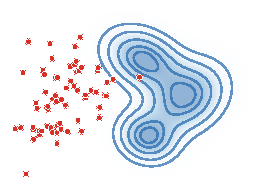
\includegraphics[width=.178\linewidth]{figures/semidiscrete-lloyd-flow-mixtures/snapshot-000.pdf} &
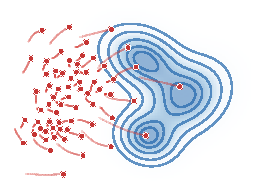
\includegraphics[width=.178\linewidth]{figures/semidiscrete-lloyd-flow-mixtures/snapshot-024.pdf} &
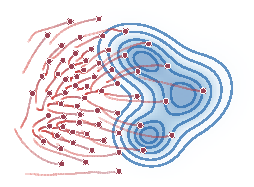
\includegraphics[width=.178\linewidth]{figures/semidiscrete-lloyd-flow-mixtures/snapshot-080.pdf} &
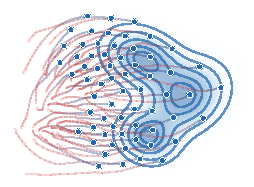
\includegraphics[width=.178\linewidth]{figures/semidiscrete-lloyd-flow-mixtures/snapshot-240.pdf} &
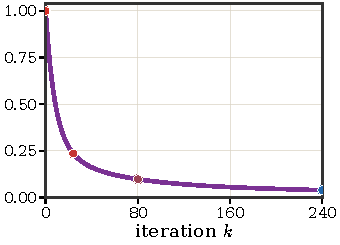
\includegraphics[width=.220\linewidth]{figures/semidiscrete-lloyd-flow-mixtures/energy-decay.pdf}
\end{tabular}
\caption{\emph{Relaxed Lloyd flow from a source Gaussian-mixture initialization toward a different target Gaussian-mixture density.} The blue contours and shading show the target density \(\al\), while the colored disks are the moving codepoints initialized from the source mixture. The faint curves trace the labelled sites under the explicit-Euler Lloyd ODE. The right panel displays the relative quantization energy \(\Ff(Y^{(k)})/\Ff(Y^{(0)})\), illustrating the monotone decay of the objective along the relaxed iterations.}
\index{Lloyd!flow}% strictindex
\index{quantization!energy}% strictindex
\index{Gaussian!mixture}% strictindex
\label{fig:semidiscrete-lloyd-flow-mixtures}
\end{figure}

\begin{alg}[Lloyd quantization]\label{alg:lloyd-quantization}
\textbf{Input:} Source measure $\al$, initial codepoints $Y^{(0)}=(y_j^{(0)})_{j=1}^m$, squared Euclidean cost, tolerance $\mathrm{tol}$, iteration budget $K\geq1$.

\textbf{Output:} Codepoints $Y=(y_j)_{j=1}^m$.

\textbf{Initialize:} Set \(d_0=+\infty\) and \(k=0\).

\textbf{While} \(d_k>\mathrm{tol}\) and $k<K$ \textbf{do}:
\begin{algblock}

\textbf{Set} \(k\leftarrow k+1\).

\textbf{Compute the tie-broken Voronoi partition:}
\(\VV_j(Y^{(k-1)}) = \enscond{x}{j=\min\argmin_{1\leq \ell\leq m}\norm{x-y_\ell^{(k-1)}}^2}.\)

\textbf{For} each nonempty cell $\VV_j$ \textbf{do}:
\begin{algblock}
\(y_j^{(k)} = \frac{\int_{\VV_j(Y^{(k-1)})}x\,\d\al(x)} {\int_{\VV_j(Y^{(k-1)})}\d\al(x)}.\)
\end{algblock}
\textbf{For} each empty cell $\VV_j$ \textbf{do}:
\begin{algblock}

\textbf{Set} $y_j^{(k)}=y_j^{(k-1)}$.

\end{algblock}

\textbf{Set} \(d_k=\max_j\norm{y_j^{(k)}-y_j^{(k-1)}}\).
\end{algblock}
\algreturnskip
\textbf{Return} $Y^{(k)}$.
\end{alg}

Figure~\ref{fig:semidiscrete-lloyd-quantization} follows the associated Voronoi cells and generators through Lloyd iterations, making the decrease of the quantization energy visible.

\begin{figure}[H]
\centering
\begin{tabular}{@{}ccc@{}}
\small initialization &
\small after $6$ iterations &
\small after $36$ iterations \\[-.15em]

\includegraphics[width=.30\linewidth]{figures/semidiscrete-lloyd-quantization/initial.pdf} &
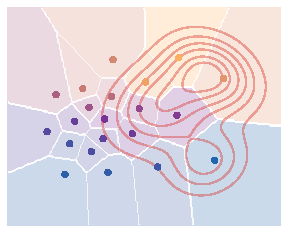
\includegraphics[width=.30\linewidth]{figures/semidiscrete-lloyd-quantization/iter6.pdf} &
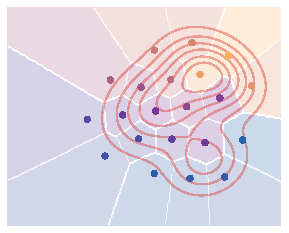
\includegraphics[width=.30\linewidth]{figures/semidiscrete-lloyd-quantization/iter36.pdf}
\end{tabular}
\caption{\emph{Lloyd quantization for the same continuous density and twenty-one initial sites as Figure~\ref{fig:semidiscrete-laguerre-cells}.} The red contours show the density $\al$, while the colored disks are the current codepoints and have the same colors as their Voronoi cells. The iterations move the initially left-located sites toward the high-density region and reshape the cells according to centroidal Voronoi geometry.}
\index{centroidal Voronoi}% strictindex
\index{Laguerre cell}% strictindex
\index{Voronoi cell}% strictindex
\label{fig:semidiscrete-lloyd-quantization}
\end{figure}

\paragraph{Quantization with fixed equal weights.}
\index{quantization!fixed weights}% strictindex
\index{Wasserstein!gradient flow}% strictindex
The free-mass formulation above optimizes the positions and the weights of the atoms. A different problem is obtained by prescribing the weights. In the equal-weight case, set
\[
	\nu_Y\eqdef \frac1m\sum_{j=1}^m\de_{y_j},
	\qquad
	\Ff_{\rm eq}(Y)
	\eqdef
	\frac12\Wass_2^2(\al,\nu_Y),
	\]
and minimize only over the positions \(Y=(y_j)_j\). Assume that the sites are distinct, that \(\al\) has a density, and that it does not charge the boundaries of the semi-discrete optimal cells. Let \(C_j(Y)\) be the Laguerre cell transported to \(y_j\), so that \(\al(C_j(Y))=1/m\), and define its centroid
\[
	\bar x_j(Y)
	\eqdef
	m\int_{C_j(Y)} x\d\al(x).
\]
At differentiability points, the envelope theorem gives
\[
	\nabla_{y_j}\Ff_{\rm eq}(Y)
	=
	\frac1m\bigl(y_j-\bar x_j(Y)\bigr).
\]
As long as the optimal matching between two nearby labelled configurations preserves labels, the \(\Wass_2\) metric on equal-weight empirical measures induces the local particle metric \(g_Y(U,V)=m^{-1}\sum_j\dotp{u_j}{v_j}\). Hence the associated \(\Wass_2\) gradient flow is the coupled system
\[
	\dot y_j(t)
	=
	\bar x_j(Y_t)-y_j(t),
	\qquad j=1,\ldots,m.
\]
Equivalently, \(\nu_{Y_t}\) satisfies a continuity equation with velocity \(v_t(y_j(t))=\bar x_j(Y_t)-y_j(t)\). This is the so-called finite-particle \(\Wass_2\) gradient-flow viewpoint developed more systematically in Chapter~\ref{sec-wasserstein-gradient-flows}; the fixed-weight cells are Laguerre cells rather than the free-mass Voronoi cells used by Lloyd's method.

\paragraph{Equal-weight quantization on the line.}
The following classical scalar quantization result gives the precise form of the inverse-CDF rule for equal-weight quadratic quantization; see~\cite{graf2000foundationsquantization}. The atoms are not exactly the midpoint quantiles in general; they are the averages of the quantile function over equal mass bins. Midpoint inverse-CDF samples are nevertheless asymptotically equivalent and are often the most convenient rule in numerical examples. For the uniform law on $[0,1]$, both rules coincide and give the regular grid $y_i=(i-1/2)/m$.
\index{quantile!quantization}% strictindex
\index{empirical!measure}% strictindex

\begin{prop}[One-dimensional equal-weight quantization]\label{prop-1d-equal-weight-quantization}
	Let $\al\in\Mm_+^1(\RR)$ have finite second moment and quantile function $Q=\cumul{\al}^{-1}$. For
	\[
		\Qq^{\mathrm{eq}}_m(\al)^2
		\eqdef
		\min_{y_1\leq\cdots\leq y_m}
		\Wass_2^2\left(\al,\frac1m\sum_{i=1}^m\de_{y_i}\right),
	\]
	set $I_i=((i-1)/m,i/m]$. Then the sorted minimizer is unique and its $i$th atom is
	\[
		y_i^\star
		=
		m\int_{I_i} Q(u)\d u,
	\]
	and
	\[
		\Qq^{\mathrm{eq}}_m(\al)^2
		=
		\sum_{i=1}^m
		\int_{I_i}
		\abs{Q(u)-y_i^\star}^2\d u.
	\]
	If $Q\in C^1([0,1])$, then
	\[
		m^2\Qq^{\mathrm{eq}}_m(\al)^2
		\longrightarrow
		\frac1{12}\int_0^1\abs{Q'(u)}^2\d u.
	\]
\end{prop}
\begin{proof}
	After sorting the atoms, the quantile formula for $\Wass_2$ gives
	\[
		\Wass_2^2\left(\al,\frac1m\sum_{i=1}^m\de_{y_i}\right)
		=
		\sum_{i=1}^m
		\int_{I_i}\abs{Q(u)-y_i}^2\d u.
	\]
	The minimization therefore decouples over the intervals $I_i$, and the best constant approximation of $Q$ on $I_i$ in $L^2$ is its average on $I_i$. Since $Q$ is nondecreasing, these interval averages are nondecreasing, so they satisfy the sorting constraint. Strict convexity in each scalar $y_i$ proves uniqueness and gives the displayed energy.

	Denote by $\bar Q_{I_i}=m\int_{I_i}Q(u)\d u$ the interval average. If $Q$ is $C^1$, set $h=1/m$ and write $I_i=(a_i,a_i+h]$. Uniform Taylor expansion gives, for $v\in[0,1]$,
	\[
		Q(a_i+hv)=Q(a_i)+hvQ'(a_i)+h\,r_i(v),
		\qquad
		\max_i\sup_{v\in[0,1]}\abs{r_i(v)}\to0.
	\]
	Subtracting the average over $v\in[0,1]$ and integrating gives
	\[
		\int_{I_i}\abs{Q(u)-\bar Q_{I_i}}^2\d u
		=
		\frac{h^3}{12}\abs{Q'(a_i)}^2+o(h^3),
	\]
	uniformly in $i$. Summing over $i$ yields a Riemann sum for $\frac1{12}\int_0^1\abs{Q'(u)}^2\d u$.
\end{proof}

Thus the common deterministic rule $m^{-1}\sum_i\de_{Q((i-1/2)/m)}$ should be read as a midpoint approximation of the optimal bin-average formula. It has the same leading squared error under the same smoothness assumptions. Indeed, orthogonal projection onto constants on each $I_i$ gives
\[
	\int_{I_i}|Q(u)-z|^2\d u
	=
	\int_{I_i}|Q(u)-y_i^\star|^2\d u
	+
	\frac1m|z-y_i^\star|^2,
\]
and $Q((i-1/2)/m)-y_i^\star=o(m^{-1})$ uniformly when $Q\in C^1([0,1])$. Random sampling has a different asymptotic regime.
\index{empirical!OT rate}% strictindex

\begin{prop}[Quantile-process asymptotics for random placement]\label{prop-1d-random-quantile-process}
\index{quantile!process}% strictindex
\index{Brownian bridge}% strictindex
	Let $\al\in\Mm_+^1(\RR)$ have quantile $Q\in C^1([0,1])$, and let $\widehat\al_m=m^{-1}\sum_{i=1}^m\de_{X_i}$ with $X_i$ i.i.d. with law $\al$. If $B$ denotes the standard Brownian bridge on $[0,1]$, then
	\[
		m\,\Wass_2^2(\al,\widehat\al_m)
		\overset{\mathrm{law}}{\longrightarrow}
		\int_0^1 B(u)^2\abs{Q'(u)}^2\d u,
	\]
	and, in expectation,
	\[
		m\,\EE\!\left[\Wass_2^2(\al,\widehat\al_m)\right]
		\longrightarrow
		\int_0^1 u(1-u)\abs{Q'(u)}^2\d u.
	\]
\end{prop}
\begin{proof}
	Let $\widehat Q_m$ be the empirical quantile function. The one-dimensional formula gives
	\[
		\Wass_2^2(\al,\widehat\al_m)
		=
		\int_0^1\abs{\widehat Q_m(u)-Q(u)}^2\d u.
	\]
	Write $X_i=Q(U_i)$ with $U_i$ i.i.d. uniform on $[0,1]$, and let $\widehat U_m^{-1}$ be the empirical quantile function of the $U_i$. Then $\widehat Q_m=Q\circ \widehat U_m^{-1}$. The classical uniform quantile-process theorem~\cite{vanDerVaartWellner1996,BobkovLedoux2019EmpiricalKantorovich} gives
	\[
		\sqrt m\,(\widehat U_m^{-1}-\Id)
		\overset{\mathrm{law}}{\longrightarrow}
		-B
		\quad\text{in }L^2(0,1).
	\]
	Because $Q'$ is uniformly continuous and $\widehat U_m^{-1}\to\Id$ uniformly in probability, the functional delta method gives
	\[
		\sqrt m\,(\widehat Q_m-Q)
		\overset{\mathrm{law}}{\longrightarrow}
		-B\,Q'
		\quad\text{in }L^2(0,1).
	\]
	Since $B$ and $-B$ have the same law, the sign disappears in the squared $L^2$ norm. The continuous mapping theorem gives the distributional convergence. Standard fourth-moment bounds for the uniform quantile process, together with the boundedness of $Q'$, give uniform integrability of the squared $L^2$ norms and hence convergence of expectations. Since $\EE[B(u)^2]=u(1-u)$, Fubini's theorem gives the displayed expectation limit.
\end{proof}

Combining Propositions~\ref{prop-1d-equal-weight-quantization} and~\ref{prop-1d-random-quantile-process}, one obtains a sharp contrast between optimal placement and random placement on the line. Deterministic equal-weight quantization has squared error of order $m^{-2}$, hence $\Wass_2$ error of order $m^{-1}$, while i.i.d. empirical sampling has expected squared error of order $m^{-1}$, hence root-mean-square $\Wass_2$ error of order $m^{-1/2}$. This one-dimensional comparison is consistent with the broader empirical OT sample-complexity theory~\cite{dereich2013constructive,fournier2015rate,weed2017sharp}.

Figure~\ref{fig:semidiscrete-quantile-quantization-rates} illustrates both parts of this comparison: optimal atoms are uniform in quantile coordinates, and their error decays one power of $m$ faster than the root-mean-square empirical error.

\begin{figure}
\centering
\begin{tabular}{cc}
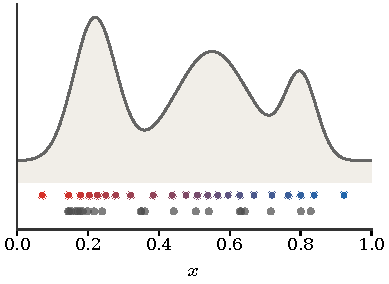
\includegraphics[width=.43\linewidth]{figures/semidiscrete-quantile-quantization-rates/quantile-points.pdf} &
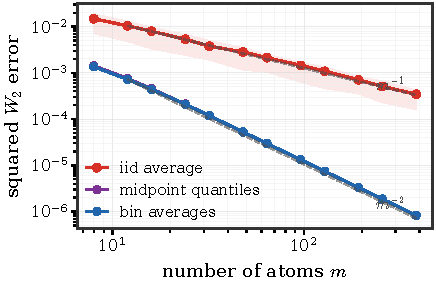
\includegraphics[width=.43\linewidth]{figures/semidiscrete-quantile-quantization-rates/rate-comparison.pdf}
\\[-.2em]
\small equal-mass quantile particles &
\small deterministic versus i.i.d. decay
\end{tabular}
\caption{\emph{One-dimensional equal-weight quantization in quantile coordinates.} Left: for a smooth positive density on $[0,1]$, the colored atoms are bin averages of the inverse CDF over equal quantile intervals, while the gray atoms show one i.i.d. empirical draw with the same number of particles. Right: expected squared $\Wass_2$ errors. The deterministic bin averages and midpoint quantiles follow the $m^{-2}$ squared-error law, whereas i.i.d. empirical measures follow the slower $m^{-1}$ expected squared-error law.}
\label{fig:semidiscrete-quantile-quantization-rates}
\end{figure}




%%%%%%%%%%%%%%%%%%%%%%%%%%%%%%%%%%%%%%%%%%%%%%%%%%%%%%%%%%%%%%%%%%%%%%%%%%%
\section[W1]{Wasserstein-1 norm}
\index{norm!Wasserstein-1}% strictindex
\label{sec-W1}

The $\Wass_1$ distance has an especially transparent dual: the admissible potentials are exactly $1$-Lipschitz test functions. This makes $\Wass_1$ the meeting point between transport, PDE formulations and weak norms on signed measures.
\index{signed!measure}% strictindex

\paragraph{$c$-transform for $\Wass_1$.}
\index{c-transform}% strictindex

Assume that $d$ is a distance on $\X=\Y$ and take the ground cost $c(x,y)=d(x,y)$. We denote the Lipschitz constant of $f\in\Cc(\X)$ by
\index{ground cost}% strictindex
\index{Lipschitz!constant}% strictindex
\begin{defn}[Lipschitz constant]\label{def-lipschitz-constant}
	For a function $f:\X\to\RR$ on a metric space $(\X,d)$, its Lipschitz constant is
	\eql{\label{eq-lip-constant}
		\Lip(f)
		\eqdef
		\sup\enscond{\frac{|f(x)-f(y)|}{d(x,y)}}{x\neq y}.
	}
	The function is $1$-Lipschitz when $\Lip(f)\leq1$.
\end{defn}

\begin{prop}[$c$-transforms and $1$-Lipschitz functions]\label{prop-w1-c-transform-lipschitz}
\index{c-transform}% strictindex
\index{Lipschitz!function}% strictindex
	Suppose $\X=\Y$ and $c(x,y)=d(x,y)$. Then there exists $g$ such that $f=g^c$ if and only if $\Lip(f)\leq1$. Furthermore, if $\Lip(f)\leq1$, then $f^c=-f$.
\end{prop}
\begin{proof}
	First suppose $f=g^c$ for some $g$. For $x,y\in\X$,
	\[
		|f(x)-f(y)|
		=
		\left|\inf_z[d(x,z)-g(z)]-\inf_z[d(y,z)-g(z)]\right|
		\leq
		\sup_z |d(x,z)-d(y,z)|
		\leq d(x,y),
	\]
	where the last inequality is the reverse triangle inequality. Thus $\Lip(f)\leq1$.
\index{triangle inequality}% strictindex

	If $\Lip(f)\leq1$, then $f(x)\leq f(y)+d(x,y)$, so $d(x,y)-f(x)\geq -f(y)$ for all $x$ and hence $f^c(y)\geq -f(y)$. Taking $x=y$ gives $f^c(y)\leq -f(y)$. Therefore $f^c=-f$. Applying the same property to $-f$ gives $(-f)^c=f$, so every $1$-Lipschitz function is $c$-concave.
\index{Lipschitz!function}% strictindex
\end{proof}

By Proposition~\ref{prop-w1-c-transform-lipschitz}, a closed dual pair has the form $(f,-f)$ with $\Lip(f)\leq1$. The Kantorovich dual therefore becomes the Kantorovich--Rubinstein formula
\index{Kantorovich-Rubinstein@Kantorovich--Rubinstein!formula}% strictindex
\index{c-transform}% strictindex
\eql{\label{eq-w1-metric}
	\Wass_1(\al,\be)
	=
	\umax{f}
	\enscond{\int_\X f\d(\al-\be)}{\Lip(f)\leq1}
	=:
	\norm{\al-\be}_{W_1}.
}
This expression depends only on the signed measure $\xi=\al-\be$. On compact $\X$, it therefore extends to every finite signed measure $\xi$ with $\xi(\X)=0$ by the same supremum and defines the Kantorovich--Rubinstein norm $\norm{\cdot}_{W_1}$~\cite{kantorovich1958space}. Homogeneity and the triangle inequality follow directly from the supremum, while definiteness follows because Lipschitz functions separate finite Radon measures. On a noncompact pointed metric space, one uses $1$-Lipschitz functions normalized at the base point and signed measures with finite first moment.
\index{signed!measure}% strictindex
\index{Kantorovich-Rubinstein@Kantorovich--Rubinstein!norm}% strictindex

For a discrete signed measure $\al-\be=\sum_{k=1}^N r_k\de_{z_k}$ on distinct sites, with $\sum_k r_k=0$,~\eqref{eq-w1-metric} becomes the finite-dimensional linear program
\index{finite-dimensional linear program}% strictindex
\eql{\label{eq-w1-discr}
	\Wass_1(\al,\be)
	=
	\umax{(f_k)_k}
	\enscond{\sum_k f_k r_k}{\foralls k,\ell,\ |f_k-f_\ell|\leq d(z_k,z_\ell)}.
}
This linear program can be solved by generic interior-point or first-order methods. If $N$ support points are involved, however, it still contains $O(N^2)$ Lipschitz constraints, mirroring the $O(nm)$ coupling variables of the original discrete Kantorovich LP; the dual formulation alone does not remove the all-pairs structure. The gain comes on structured metric spaces where the distance is generated locally: it is then enough to impose Lipschitz inequalities on neighboring pairs, because summing along paths recovers the constraints between arbitrary points. The one-dimensional ordered case is the first example; the graph-geodesic case is described later in Proposition~\ref{prop-graph-w1-beckmann}.
When $d(x,y)=|x-y|$ on $\RR$, ordering the support points $z_1\leq z_2\leq\cdots$ reduces the constraints to neighboring pairs,
\[
	\Wass_1(\al,\be)
	=
	\umax{(f_k)_k}
	\enscond{\sum_k f_k r_k}{\foralls k,\ |f_{k+1}-f_k|\leq z_{k+1}-z_k}.
\]
In one dimension this is equivalent to the cumulative formula~\eqref{eq-w1-1d}.

\paragraph{$\Wass_1$ on Euclidean spaces.}

In Euclidean space, the global Lipschitz condition has a local differential form, and its dual variable is a flux. This turns the static coupling problem into a divergence-constrained convex problem.

Let $\al,\be\in\Mm_+^1(\RR^d)$ have finite first moments and set $\xi=\al-\be$. Rademacher's theorem identifies $1$-Lipschitz functions with locally Sobolev functions whose Euclidean gradient has norm at most one almost everywhere. Hence
\index{Kantorovich-Rubinstein@Kantorovich--Rubinstein!formula}% strictindex
\eql{\label{eq-w1-cont}
	\Wass_1(\al,\be) =
	\usup{f\in W_{\mathrm{loc}}^{1,\infty}(\RR^d)}
	\enscond{ \int_{\RR^d} f\d\xi }{ \norm{\nabla f}_{L^\infty(\RR^d)} \leq 1 }.
}

The correct flux space is generally not $L^1(\RR^d;\RR^d)$. For instance, transporting one Dirac mass to another produces a flux concentrated on a segment. Let $\Mm(\RR^d;\RR^d)$ denote the finite $\RR^d$-valued Radon measures, write $|\flow|$ for total variation, and define divergence distributionally by
\[
	\langle\diverg\flow,\varphi\rangle
	\eqdef
	-\int_{\RR^d}\dotp{\nabla\varphi}{\d\flow},
	\qquad \varphi\in C_c^1(\RR^d).
\]

This yields the Beckmann problem with signed source $\al-\be$.
\begin{defn}[Beckmann problem]\label{def-beckmann-problem}
For $\al,\be\in\Mm_+^1(\RR^d)$, define
\[
    \operatorname{Beck}(\al,\be)
    \eqdef
    \inf_{\flow\in\Mm(\RR^d;\RR^d)}
    \enscond{|\flow|(\RR^d)}{\diverg\flow=\al-\be}.
\]
\end{defn}

\begin{prop}[Euclidean Beckmann formula]\label{prop-euclidean-beckmann}
\index{Beckmann!formulation}% strictindex
	For $\al,\be\in\Mm_+^1(\RR^d)$ with finite first moments,
\eql{\label{eq-w1-cont-div}
	\Wass_1(\al,\be)=\operatorname{Beck}(\al,\be).
}
	If $\flow=w\,\d x$ has a Lebesgue density, its cost reduces to $\int_{\RR^d}\norm{w(x)}_2\d x$.
\end{prop}
\begin{proof}
	Let $\flow$ be feasible. For a smooth $1$-Lipschitz test function,
	\[
		\int f\d(\al-\be)
		=
		-\int\dotp{\nabla f}{\d\flow}
		\leq
		|\flow|(\RR^d).
	\]
	Truncation followed by mollification approximates normalized Lipschitz functions by smooth test functions without increasing the gradient bound asymptotically. Equation~\eqref{eq-w1-cont} therefore gives $\Wass_1(\al,\be)\leq|\flow|(\RR^d)$.

	Conversely, let $\pi$ be an optimal coupling and define a vector measure by its action on $\zeta\in C_c(\RR^d;\RR^d)$:
	\[
		\int\dotp{\zeta(z)}{\d\flow(z)}
		\eqdef
		\int_{\RR^d\times\RR^d}\int_0^1
		\dotp{\zeta((1-t)x+ty)}{y-x}\d t\d\pi(x,y).
	\]
	For $\varphi\in C_c^1(\RR^d)$, the fundamental theorem of calculus gives
	\[
		\langle\diverg\flow,\varphi\rangle
		=
		-\int\!\int_0^1
		\dotp{\nabla\varphi((1-t)x+ty)}{y-x}\d t\d\pi(x,y)
		=
		\int\varphi\d(\al-\be).
	\]
	Moreover, $|\flow|(\RR^d)\leq\int\norm{x-y}_2\d\pi(x,y)=\Wass_1(\al,\be)$. Together with the first inequality, this proves equality and attainment.
\end{proof}

This is the Beckmann formulation~\cite{Beckmann52,SantambrogioBook}. The vector measure $\flow$ describes the oriented amount of mass crossing each region. On open sets disjoint from the source and target mass, $\diverg\flow=0$, which is the local conservation law.
\index{support}% strictindex

Finite-element or finite-volume discretizations of~\eqref{eq-w1-cont-div} produce nonsmooth convex programs. The same formulation extends to complete Riemannian manifolds by replacing straight segments with minimizing geodesics and using tangent-valued Radon measures together with the Riemannian divergence. If geodesics are nonunique, one chooses a measurable minimizing geodesic for almost every transported pair.

\paragraph{Graph distances and Beckmann flows.}
Finite graphs give a simple discrete instance where a metric is generated by local moves, so the all-pairs Lipschitz constraints collapse to edge constraints.

\begin{defn}[Graph geodesic distance]\label{def-graph-geodesic-distance}
\index{graph!geodesic distance}% strictindex
	Let $G=(V,E)$ be a connected finite graph with positive edge lengths $(\ell_e)_{e\in E}$. The graph geodesic distance between two vertices is
	\[
		d_G(i,j)=\min_{\gamma:i\leadsto j}\sum_{e\in\gamma}\ell_e.
	\]
	The minimum is over all paths $\gamma$ joining $i$ to $j$.
\end{defn}
This graph distance turns $\Wass_1$ into a finite-dimensional flow problem.

\begin{prop}[$\Wass_1$ and Beckmann flow on a graph]\label{prop-graph-w1-beckmann}
\index{Beckmann!flow}% strictindex
	Let $G=(V,E)$ be a connected finite graph with positive edge lengths $(\ell_e)_{e\in E}$ and graph geodesic distance $d_G$.
	For two probability vectors $\a,\b$ on $V$, set $r=\a-\b$ and orient each edge $e=(i,j)$. If
	\[
		(\nabla_G f)_e=f_j-f_i,\qquad
		\operatorname{div}_G=-\nabla_G^*
	\]
	are the finite-difference gradient and its negative adjoint, then a positive flow on the oriented edge $i\to j$ has positive divergence at $i$ and negative divergence at $j$. With this convention,
	\[
		\Wass_{1,G}(\a,\b)
		=
		\max_f \enscond{\sum_{i\in V} f_i r_i}{|f_i-f_j|\leq \ell_e\quad\forall e=(i,j)}
		=
		\min_m \enscond{\sum_{e\in E}\ell_e |m_e|}{\operatorname{div}_G m=r}.
	\]
	The vector $m_e$ is an oriented edge flow, and the constraint $\operatorname{div}_G m=r$ is conservation of mass at each vertex.
\end{prop}

\begin{proof}
	The edge constraints imply, by summing along every path and then minimizing over paths, that $|f_i-f_j|\leq d_G(i,j)$ for all vertices. Conversely, any $1$-Lipschitz function for $d_G$ satisfies $|f_i-f_j|\leq d_G(i,j)\leq\ell_e$ on every edge. The first equality is therefore the Kantorovich--Rubinstein formula on the metric space $(V,d_G)$.
\index{Kantorovich-Rubinstein@Kantorovich--Rubinstein!formula}% strictindex
\index{Lipschitz!function}% strictindex

	For the second equality, write the graph Beckmann problem and dualize its equality constraint with a potential $f$:
\index{equality constraint}% strictindex
\index{Beckmann!problem on graphs}% strictindex
	\[
		\inf_m \sum_e\ell_e|m_e|
		+\sup_f \sum_i f_i(r_i-(\operatorname{div}_G m)_i).
	\]
	Using $\operatorname{div}_G=-\nabla_G^*$, the coupling term is $\sum_e m_e(\nabla_G f)_e$. The minimization over each scalar flow $m_e$ is finite exactly when $|(\nabla_G f)_e|\leq\ell_e$, and is then equal to zero. The dual problem is therefore precisely the graph Lipschitz dual above. Strong duality holds because this is a finite-dimensional linear program with a nonempty feasible set: connectedness and $\sum_i r_i=0$ allow the signed surplus to be routed along paths. This proves the graph Beckmann formula.
\index{duality!strong}% strictindex
\index{finite-dimensional linear program}% strictindex
\index{dual!problem}% strictindex
\end{proof}

Figure~\ref{fig:w1-graph-transport-flow} shows the optimal edge flux on both a quasi-regular and a nonuniform Delaunay graph, emphasizing that the Beckmann variables live only on graph edges.

\begin{figure}[H]
\centering
\begin{tabular}{@{}cc@{}}
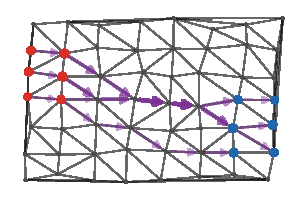
\includegraphics[width=.46\linewidth]{figures/w1-graph-transport-flow/regular.pdf}
&
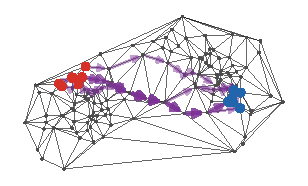
\includegraphics[width=.46\linewidth]{figures/w1-graph-transport-flow/nonuniform.pdf}
\\[-.5mm]
{\small quasi-regular Delaunay graph}
&
{\small denser nonuniform Delaunay graph}
\end{tabular}
\index{graph!transport}% strictindex
\caption{\emph{Graph Beckmann formulation of $\Wass_1$ on two Delaunay graphs $G=(V,E)$.} The left panel uses a quasi-regular vertex set, while the right panel uses a denser nonuniform vertex set sampled from a two-component Gaussian mixture. Red and blue disks encode the positive and negative parts of $r=\a-\b$, localized on six vertices each. The darker graph edges show the triangulation, while the violet arrows display the optimal signed edge flow $m$: orientation gives the sign, width is proportional to $\sqrt{|m_e|}$, and the flow satisfies $\operatorname{div}_G m=r$.}
\index{signed!positive part}% strictindex
\index{signed!negative part}% strictindex
\index{Beckmann!formulation}% strictindex
\label{fig:w1-graph-transport-flow}
\end{figure}

\begin{rem}[Sparse LP and network simplex]\label{rem-graph-w1-network-simplex}
\index{sparse linear program}% strictindex
\index{network simplex}% strictindex
	Let $N=|V|$ and $M=|E|$. The graph Beckmann problem is a linear program, but it is much smaller than the dense Kantorovich LP on the same vertex set. Indeed, writing $m=m^+-m^-$ gives
\index{Beckmann!problem on graphs}% strictindex
	\[
		\min_{m^+,m^-\geq0}\sum_{e\in E}\ell_e(m^+_e+m^-_e)
		\quad\text{subject to}\quad
		\operatorname{div}_G(m^+-m^-)=r .
	\]
	This formulation has $2M$ nonnegative variables and $N-1$ independent balance constraints, whereas the standard transport LP between two measures on $V$ has $N^2$ coupling variables and $2N-1$ independent marginal constraints. For sparse geometric graphs, such as planar Delaunay graphs where typically $M=O(N)$, the graph formulation is therefore linear-size rather than quadratic-size.
\index{Delaunay graph}% strictindex
\index{marginal!constraint}% strictindex

	The same LP is a minimum-cost transshipment problem. Replace each undirected edge $\{i,j\}$ by the two directed arcs $i\to j$ and $j\to i$, both with cost $\ell_e$, and impose the node balances $\sum_{j}u_{ij}-\sum_j u_{ji}=r_i$. This is exactly the setting of the network simplex method: a basis is a spanning tree, a pivot adds one non-tree arc, creates a unique cycle, sends flow along this cycle, and updates the node potentials and reduced costs~\cite{bertsekas1988dual,Orlin1997}. A basic implementation needs $O(M)$ work to price all arcs and $O(N)$ work to update the tree at each pivot, hence $O(PM)$ arithmetic operations for $P$ pivots on a sparse graph. The pivot count $P$ depends on the rule and can be large in worst-case simplex analyses, but network-simplex variants and general minimum-cost-flow algorithms give polynomial guarantees in $N$ and $M$; in practice, this edge-based formulation is often far cheaper than solving the dense $N^2$-variable transport LP.
\index{flow!minimum-cost}% strictindex
\index{spanning tree}% strictindex
\index{cost!reduced}% strictindex
\index{network simplex}% strictindex
\end{rem}

This graph formulation is the transshipment version of $\Wass_1$. It is the natural discrete analogue of~\eqref{eq-w1-cont-div}: gradients are edge differences, divergences are incidence-matrix balances, and geodesic distance is the shortest-path length. It can be solved by min-cost flow methods on sparse graphs, and entropic or KL-projection variants lead to flow-Sinkhorn algorithms for graph $\Wass_1$~\cite{Beckmann52,peyre2026robust}.
\index{integral probability metric}% strictindex
\index{Sinkhorn!algorithm}% strictindex
\index{matrix!incidence}% strictindex
\index{KL!projection}% strictindex
